\documentclass[
% preprint,
% preprintnumbers,
 amsmath,amssymb,
 aps,
 pre,
 longbibliography,
 10pt, onecolumn,
 notitlepage
]{revtex4-1}


\usepackage{graphicx}% Include figure files
%\graphicspath{{./figures/}} % path to figures
\usepackage{dcolumn}% Align table columns on decimal point
\usepackage{bm}% bold math
\usepackage{hyperref}% add hypertext capabilities
\usepackage{physics} % package for physics symbols

% % for referencing main.tex (c.f. xr-package example)
% \usepackage{xr}
% \makeatletter
% \newcommand*{\addFileDependency}[1]{% argument=file name and extension
%   \typeout{(#1)}
%   \@addtofilelist{#1}
%   \IfFileExists{#1}{}{\typeout{No file #1.}}
% }
% \makeatother

% \newcommand*{\myexternaldocument}[1]{%
%     \externaldocument{#1}%
%     \addFileDependency{#1.tex}%
%     \addFileDependency{#1.aux}%
% }
% \myexternaldocument{main}


\begin{document}
% define commands
\newcommand{\eqnname}{Eq.}
\newcommand{\secname}{Sec.}
% adding S prefix
\renewcommand{\theequation}{S\arabic{equation}}
\renewcommand{\thefigure}{S\arabic{figure}}
\renewcommand{\bibnumfmt}[1]{[S#1]}
\renewcommand{\citenumfont}[1]{S#1}


\title{Supplemental Material: Rectification of energy and motion in non-equilibrium parity violating metamaterials}


\author{Zhenghan Liao}
\affiliation{Department of Chemistry, University of Chicago, Chicago, IL, 60637, USA}
\author{William T. M. Irvine}
\affiliation{Department of Physics, University of Chicago, Chicago, IL 60637, USA}
\affiliation{James Franck Institute, University of Chicago, Chicago, IL 60637, USA}
\affiliation{ Enrico Fermi Institute, University of Chicago, Chicago, IL, 60637, USA}
\author{Suriyanarayanan Vaikuntanathan}
\affiliation{Department of Chemistry, University of Chicago, Chicago, IL, 60637, USA}
\affiliation{James Franck Institute, University of Chicago, Chicago, IL 60637, USA}


\maketitle

% \tableofcontents

\section{The formula for energy flux}
In this section, we derive the formula for energy flux, \eqnname~(4) in the main text.
The force $F$ in this section is a general conservative force, which does not need to be linear.
We use the following strategy to determine the energy flux. First we define the energy $E_i$ of particle $i$, and then write down an energy balance relation, that expresses the infinitesimal energy change $\dd E_i$ using stochastic calculus. Finally, we collect terms in $\dd E_i$ that couple neighboring particles together and identify this as the energy transfer among particles.

The energy of particle $i$ is defined as
\begin{equation} \label{eqnS:energy_individual}
E_i = \frac{1}{2}m_iv_i^Tv_i + U_{ii} + \frac{1}{2}\sum_{j\neq i}U_{ij},
\end{equation}
where the first term is the kinetic energy, the second term denotes the on-site potential, and the last term is the shared spring energy between the particle and its neighbors.

We use Ito's formula to calculate $\dd E_i$. 
 Ito calculus provides the advantage that the stochastic terms in $\dd E_i$ vanish under time-averaging.
For a stochastic differential equation (SDE) of variable $X$(vector) with drift $\mu$(vector) and diffusion $\sigma$(matrix)
\begin{equation} \label{eqnS:SDE_general}
\dd X = \mu \dd t + \sigma \dd W ,
\end{equation}
where $\dd W$ is a vector consisting of standard Wiener processes,
Ito's formula gives the SDE of function $f(X)$
\begin{equation} \label{eqnS:SDE_ito}
\dd f(X) = ((\nabla_X^Tf)\mu + \frac{1}{2}\tr[\sigma \sigma^T \nabla_X\nabla_X^Tf])\dd t + (\nabla_X^Tf) \sigma \dd W,
\end{equation}
where $\nabla_X$ denotes the gradient with respect to $X$, the superscript $T$ denotes the transpose, and $\tr$ denotes the trace.

We begin by writing the equation of motion of our system \eqnname~(1) in the form of a stochastic differential equation \eqnname~\eqref{eqnS:SDE_general}.
We represent $N$ particles' position by a column vector $z = \sum_{i=1}^N \ket{i}\otimes z_i$, where $\ket{i}$ denotes the 2D subspace of particle $i$. Similar representations are also applied to $v$ and $\eta$. 
Then we get
\begin{align}
X &= \pmqty{ z & v & \eta }^T, \label{eqnS:SDE_X}\\
\mu &= \pmqty{ v \\
\frac{1}{m}(-\nabla_zU - BAv - \gamma v + \eta) \\
-\frac{1}{\tau}\eta }, \label{eqnS:SDE_mu} \\
\sigma &= \text{diag} \pmqty{0 & 0 & \frac{\sqrt{2\gamma T_a}}{\tau} I}, \label{eqnS:SDE_sigma}
\end{align}
where $U$ is the total energy of the system, $A$ is an antisymmetric matrix $A=\sum_i \ket{i}\bra{i}\otimes \mqty(0 & 1 \\ -1 & 0)$, and $\text{diag}()$ means a block-diagonal matrix.

Now we apply Ito's formula \eqnname~\eqref{eqnS:SDE_ito} to our system by associating with the function $f(X)$, the energy of particle $i$, $E_i(X)$.
The nonzero terms in the gradient of $E_i$ are
\begin{align}
\nabla_{z_i}E_i &= -(F_{ii} + \frac{1}{2}\sum_jF_{ji}), \\
\nabla_{z_j}E_i &= -\frac{1}{2}F_{ij}, \\
\nabla_{v_i}E_i &= m_iv_i.
\end{align}

The term $(\nabla_X^TE_i)\mu$ reads
\begin{equation}
\begin{split}
(\nabla_X^TE_i)\mu
&= (\nabla_{z_i}^TE_i)v_i + \sum_j(\nabla_{z_j}^TE_i)v_j + (\nabla_{v_i}^TE_i)m_i^{-1}(-\nabla_{z_i}U - BAv_i - \gamma v_i + \eta_i) \\
&= -(F_{ii} + \frac{1}{2}\sum_jF_{ji})^T v_i - \sum_j\frac{1}{2}F_{ij}^T v_j + v_i^T (F_{ii} + \sum_jF_{ji}) - \gamma v_i^Tv_i + v_i^T\eta_i \\
&= -\sum_j\frac{1}{2}(v_i + v_j)^T F_{ij} - \gamma v_i^Tv_i + v_i^T\eta_i ,
\end{split}
\end{equation}
where we used $F_{ji} = -F_{ij}$ and $v_i^TAv_i = 0$.
The term $\frac{1}{2}\tr[\sigma \sigma^T \nabla_X\nabla_X^Tf]$ and $\nabla_X^Tf$ are zero.

Finally, the energy change can be written as
\begin{align}
\dd E_i &= -\sum_jJ_{ij}\dd t + h_i \dd t, \label{eqnS:flux_dEi} \\
J_{ij} &= \frac{1}{2}(v_i + v_j)^T F_{ij}, \label{eqnS:flux_Jij} \\
h_i &= -\gamma_i v_i^Tv_i +v_i^T\eta_i. \label{eqnS:flux_hi}
\end{align}
$J_{ij}$ is identified as the energy transferred per unit time from particle $i$ to $j$, and $h_i$ is identified as the energy transferred from the bath to particle $i$.

As for the steady-state average of $J_{ij}$, we use $\expval{\dd U_{ij} / \dd t =0}$ and the chain rule to simplify \eqnname~\eqref{eqnS:flux_Jij}
\begin{equation}
    0 = v_i^T F_{ji} + v_j^T F_{ij}
    = -v_i^T F_{ij} + v_j^T F_{ij},
\end{equation}
and arrive at the expresion
\begin{equation}
    \expval{J_{ij}} = \expval{v_j^T F_{ij}}.
\end{equation}


\section{Numerical method for solving the energy flux}
One straightforward numerical method to compute the flux $J$ is as follows.
Our system is determined by the network geometry and parameters $m, k_g, k, B, \gamma, \tau, T_a$.
Given the equation of motion \eqnname~\eqref{eqnS:SDE_general},\eqref{eqnS:SDE_X}-\eqref{eqnS:SDE_sigma}, one can numerically solve for the covariance $C=\expval{XX^T}$ from the matrix equation $\mu C + C \mu^T = \sigma\sigma^T$ \cite{Gardiner2009ItoCalculus,Ceriotti2010ColoredNoiseThermostats}.
Finally, the flux \eqnname~\eqref{eqnS:flux_Jij}, which is bilinear in $x$ and $v$, can be extracted from the covariance $C$.
Numerical calculations of $\expval{J}$ are performed using Mathematica with custom code \cite{WolframResearch2018MathematicaVersion}


\section{Energy flux from linear response theory}
Following \cite{Kundu2011LargeDeviations}, we derive the expression of the energy flux (\eqnname~(7) and (10) in the main text) using a spectral linear response theory.

\subsection{Fourier modes for energy flux}

We define Fourier transform (FT) of a function $f(t)$ as
\begin{align}
\tilde{f}(\omega) &= \frac{1}{t} \int_0^t dt'\ f(t')e^{-i\omega t'},\quad
\omega = \frac{2\pi n}{t} ,\\
f(t) &= \sum_{\omega=-\infty}^{\infty} \tilde{f}(\omega) e^{i\omega t} .
\end{align}

The FT of the equation of motion \eqnname~\eqref{eqnS:SDE_general},\eqref{eqnS:SDE_X}-\eqref{eqnS:SDE_sigma} reads
\begin{align}
\tilde{v}(\omega) &= i\omega \tilde{z}(\omega) ,\label{eqnS:FT_v}\\
\tilde{z}(\omega) &= G^+(\omega) \tilde{\eta}(\omega) ,\label{eqnS:FT_z}\\
\tilde{\eta}(\omega) &= \frac{\sqrt{2\gamma T_a}}{1 + i\omega \tau} \tilde{\xi}(\omega) ,\label{eqnS:FT_eta}
\end{align}
where $G^+$ is the response function
\begin{equation} \label{eqnS:response}
G^{\pm}(\omega) = [K \pm i\omega(\gamma I + BA) - m\omega^2I]^{-1} .
\end{equation}

The energy flux $J_{ij}$ from \eqnname~\eqref{eqnS:flux_Jij} can be expressed as a bilinear function in $z$ and $v$, by writing the linearized force $F$ in terms of $z$,
\begin{align}
    J_{ij} &= kv^TA^{J}z \\
    \begin{split}
    A^{J} &\equiv \frac{1}{2} (\ket{i}\bra{i} \otimes e_{ij}e_{ij}^T + \ket{i}\bra{j} \otimes e_{ij}e_{ji}^T \\
    &\quad + \ket{j}\bra{i} \otimes (-e_{ji}e_{ij}^T) + \ket{j}\bra{j} \otimes (-e_{ji}e_{ji}^T)) .
    \end{split}
\end{align}
    
This bilinear form enables us to write the time integral of energy flux $Q = \int_0^t \dd{t'} J(t')$ as a sum of Fourier modes $\tilde{q}_\omega$ using Parseval's theorem,
\begin{align}
    Q &= t\sum_{\omega=-\infty}^{\infty} \tilde{q}_\omega, \\
    q_\omega &= k\tilde{v}^T A^{J} \tilde{z}^*
    = i\omega k \tilde{\eta}^TG^{+T}A^{J}G^-\tilde{\eta}^* ,
\end{align}
where the superscript $*$ denotes the complex conjugate.

Pairing $\tilde{q}_\omega$ and its conjugate $\tilde{q}_{-\omega}$ gives a real function, which would be beneficial for subsequent derivations.
\begin{gather}
    Q = t\sum_{\omega=2\pi/t}^{\infty} (\tilde{q}_\omega + \tilde{q}_{-\omega}), \label{eqnS:qmode_sum}\\
    \tilde{q}_\omega + \tilde{q}_{-\omega} = \tilde{\eta}(\omega)^T A_\omega^q \tilde{\eta}(\omega)^* \\
    A_\omega^q = -i\omega k G^{+T}(\omega) A^{as} G^-(\omega), \\
    A^{as} = -(A^{J} - {A^{J}}^T)
    = -\ket{i}\bra{j} \otimes e_{ij}e_{ji}^T + \ket{j}\bra{i} \otimes e_{ji}e_{ij}^T.
\end{gather}

Averaging $\tilde{q}_\omega + \tilde{q}_{-\omega}$ over the noise $\tilde{\eta}(\omega)$ using the relationship between $\tilde{\eta}$ and $\tilde{\xi}$ \eqnname~\eqref{eqnS:FT_eta}, and $\expval{\tilde{\xi}(\omega) \tilde{\xi}^T(\omega')} = \frac{1}{t} I \delta(\omega + \omega')$, we get
\begin{equation} \label{eqnS:qmode_single}
\begin{split}
\expval{\tilde{q}_\omega + \tilde{q}_{-\omega}}
&= \frac{2\gamma T_a}{1 + \omega^2 \tau^2} \tr[A_\omega^q \expval{\tilde{\xi}(-\omega)\tilde{\xi}(\omega)^T}] \\
&= \frac{1}{t} \frac{2\gamma T_a}{1 + \omega^2 \tau^2} \tr A_\omega^q .
\end{split}
\end{equation}

\subsection{Integrating over the Fourier modes}

In long time limit, the sum can be approximated by an integral
\begin{equation}
\frac{1}{t} \sum_{\omega=2\pi/t}^{\infty}
= \frac{1}{2t} \sum_{\omega=-\infty}^{\infty} \frac{t \Delta\omega}{2\pi}
\approx \frac{1}{4\pi}\int_{-\infty}^{\infty} \dd{\omega} .
\end{equation}
\eqnname~\eqref{eqnS:qmode_sum} and \eqref{eqnS:qmode_single} can then be turned to an integral expression of the flux
\begin{equation} \label{eqnS:flux_integral_raw}
\expval{J} = \lim_{t\rightarrow \infty} \frac{\expval{Q}}{t}
= \frac{\gamma T_a}{2\pi} \int_{-\infty}^{\infty} \dd{\omega} \frac{\tr A_\omega^q}{1+\omega^2\tau^2} .
\end{equation}

In the next steps, we simplify this integral with the help of the property \cite{Kundu2011LargeDeviations}
\begin{equation} \label{eqnS:response_property}
G^-(\omega) - G^{+T}(\omega) = 2i\omega\gamma G^-(\omega)G^{+T}(\omega) .
\end{equation}
Using this property, the trace of $A_\omega^q$ becomes
\begin{equation}
\begin{split}
\tr A_\omega^q &= -i\omega k \tr G^{+T} A^{as} G^- \\
&= -i\omega k \frac{1}{2i\omega \gamma} \tr (G^- - G^{+T})A^{as} \\
&= -\frac{k}{\gamma} \Re\tr G^+A^{as} .
\end{split}
\end{equation}

Plugging this trace into \eqnname~\eqref{eqnS:flux_integral_raw}, we get the integral form for the flux \eqnname~(7)
\begin{equation}
\expval{J} = -\frac{T_ak}{2\pi} \int_{-\infty}^{\infty} \dd{\omega} \frac{\Re \tr G^+A^{as}}{1+\omega^2\tau^2} .
\end{equation}

This integral can be calculated using the residue theorem.
Since $\Im G^+(-\omega) = -\Im G^+(\omega)$,
$\frac{\Im \tr G^+A^{as}}{1+\omega^t\tau^2}$ is an odd function of
$\omega$, and its line integral vanishes.
\begin{equation}
\expval{J} = -\frac{T_ak}{2\pi} \int_{-\infty}^{\infty} \dd{\omega} \frac{\tr G^+A^{as}}{1+\omega^2\tau^2} .
\end{equation}
The integrand vanishes at $\omega \rightarrow \infty$, so the line
integral can be converted to a contour integral along the
counter-clockwise semicircle $R$ in the lower-half plane
\begin{equation}
\expval{J} = \frac{T_ak}{2\pi} \oint_R \dd{\omega} \frac{\tr G^+A^{as}}{1+\omega^2\tau^2} .
\end{equation}
The noise correlation $\tau$ introduces a pole of the integrand at $\omega=-i/\tau$, thus the contour integral can be evaluated as
\begin{equation} \label{eqnS:flux_residue}
\expval{J} = -\frac{T_ak}{2\tau} \tr G^+(-\frac{i}{\tau})A^{J,as} ,
\end{equation}
and the response function at $\omega=-i/\tau$ reads
\begin{equation} \label{eqnS:response_at_pole}
G^+(-\frac{i}{\tau})
= [K + (\frac{\gamma}{\tau} + \frac{m}{\tau^2})I + \frac{B}{\tau}A]^{-1} .
\end{equation}

In theory, the equation \eqnname~\eqref{eqnS:flux_residue} provides the analytical solution of the flux, because the inverse matrix \eqnname~\eqref{eqnS:response_at_pole} can be expressed analytically.
In practice, analytical solutions can be easily calculated for small networks, but are hard for large networks.
Nevertheless, some general properties of the flux can be obtained from \eqnname~\eqref{eqnS:flux_residue} after some algebra. For network with only horizontal and vertical bonds (\figurename~1b), all fluxes are zero. For two networks whose slanted bonds have opposite angles (\figurename~1b), their fluxes are opposite. Changing $B$ to $-B$ would change the flux $J$ to $-J$.


\section{Kirchoff's law}
The derivation of the Kirchoff's law is similar to the derivation of the energy flux, except that we use the energy from the bath to the particle $h_i$ in \eqnname~\eqref{eqnS:flux_hi} instead of $J_{ij}$ in \eqnname~\eqref{eqnS:flux_Jij}.

Following the procedure in the last section from \eqnname~\eqref{eqnS:qmode_sum} to \eqref{eqnS:flux_integral_raw}, we arrive at an integral expression for the $\expval{h_i}$ with a different $A_\omega^q$
\begin{gather}
    \expval{h_i} = \frac{\gamma T_a}{2\pi} \int_{-\infty}^{\infty} \dd{\omega} \frac{\tr A_\omega^q}{1+\omega^2\tau^2}, \label{eqnS:flux_hi_fourier}\\
    A_\omega^q = i\omega (G^{+T} \rho_i - \rho_iG^-) - 2\gamma\omega^2 G^{+T} \rho_i G^- ,\\
    \rho_i = \ket{i}\bra{i} .
\end{gather}

Using the property of $G^\pm$ \eqnname~\eqref{eqnS:response_property}, we get
\begin{equation}
    \begin{split}
        \tr (G^{+T} \rho_i - \rho_iG^-)
        &= \tr \rho_i(G^{+T} - G^-) \\
        &= -\tr \rho_i 2i\omega \gamma G^- G^{+T} \\
        &= -2i\omega\gamma \tr G^{+T}\rho_i G^- ,
    \end{split}
\end{equation}
so the trace of $A_\omega^q$ vanishes
\begin{equation}
    \tr A_\omega^q
    = i\omega \tr (G^{+T} \rho_i - \rho_iG^-) - \tr 2\gamma\omega^2 G^{+T} \rho_i G^-
    = 0 .
\end{equation}

From \eqnname~\eqref{eqnS:flux_hi_fourier}, $\expval{h_i}$ is also zero, so on average there is no energy exchange between the particle and the bath. Because the average change of $E_i$ is zero, and $\expval{\dot{E_i}} = -\sum_j\expval{J_{ij}} + \expval{h_i}$, we obtain the Kirchoff's law
\begin{equation}
    -\sum_j\expval{J_{ij}} = \sum_j\expval{J_{ji}} = 0 .
\end{equation}


\section{Connection to isolated gyroscopic networks}

\begin{figure}[tbp]
	\centering
	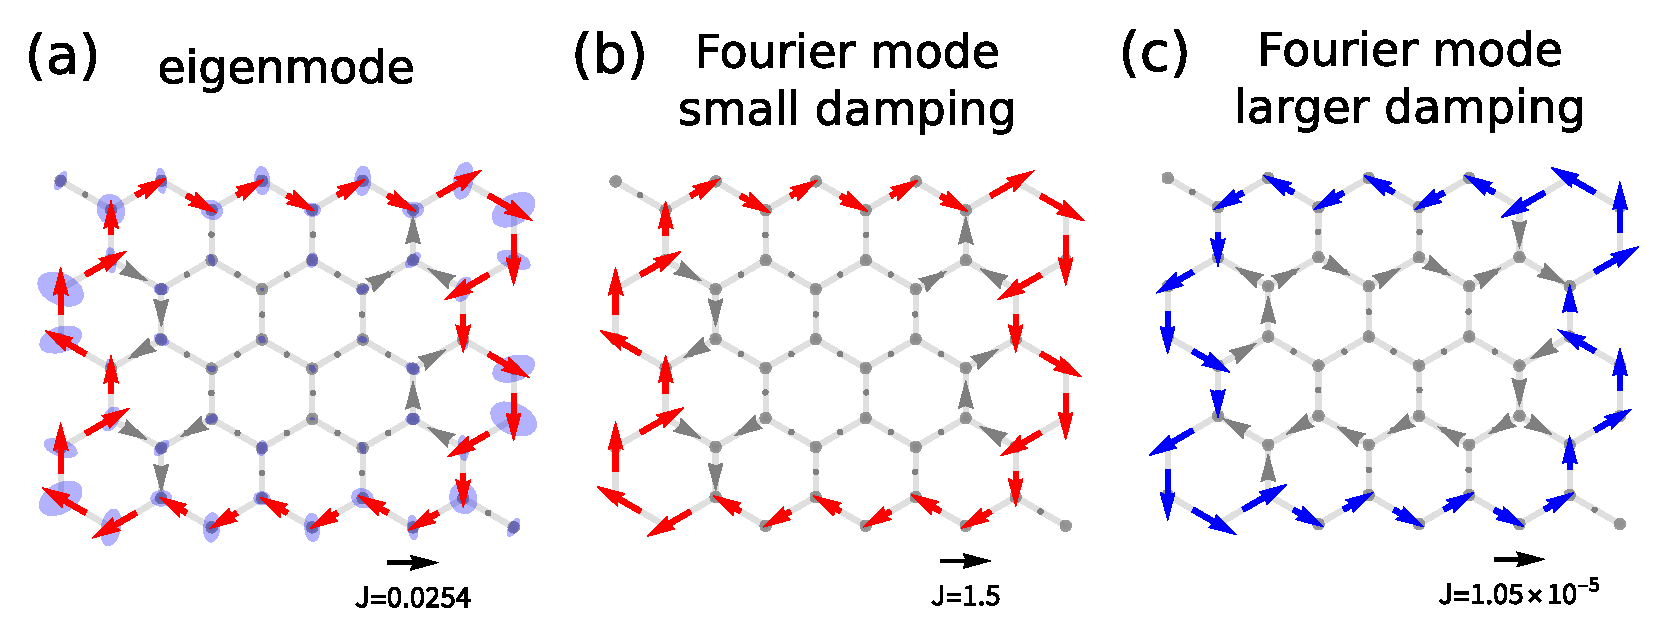
\includegraphics[width=0.8\textwidth]{Fourier_modes.pdf}
    \caption{
        Comparison between a boundary-localized eigenmode of the undamped isolated network and the Fourier modes of the damped network at the same frequency. First order dynamics (by setting $m=0$) are used. Numerical calculations are performed with all other parameters set to $1$.
        (a) Eigenmode of undamped gyroscopic system. For the frequency chosen, the eigenmode is localized on the boundary. Blue disks represent the orbit of particles.
        (b) The Fourier mode of damped variant of our model at small $\gamma$ ($\gamma=0.001$) resembles the eigenmode.
        (c) The Fourier mode at larger $\gamma$ ($\gamma=1$) is no longer close to the eigenmode.
    }
    \label{fig:Fourier_modes}
\end{figure}

Since our model is built upon the well-studied isolated system in Refs \cite{Nash2015TopologicalMechanics,Susstrunk2016ClassificationTopological,Mitchell2018AmorphousTopological,Lee2018TopologicalDynamics}, we would like to build a connection between our energy flux in the active system and eigenmodes in those studies.
In this section, we show that the flux formula \eqnname~(10) can be decomposed to a weighted sum over eigenmodes \eqnname~\eqref{eqnS:flux_eigen}. Then we apply this result to a honeycomb network as an example.

The Fourier analysis from \secname~IV in the main text is not suitable for this connection, because Fourier modes and eigenmodes are related only at small $\gamma$'s (\figurename~\ref{fig:Fourier_modes}a and b), but they become dissimilar at larger $\gamma$'s (\figurename~\ref{fig:Fourier_modes}a and c).
The underlying discrepancy between Fourier modes and eigenmodes comes from the fact that eigenmodes are a natural basis for the isolated network, whereas Fourier modes have an extra factor of friction or damping.
In addition to this extra factor $\gamma$,
the active system also has extra factors of $m$ and $\tau$. The factor $m$ comes from the order of dynamics: the active system is second order in time, while the gyroscopic dynamics in \cite{Nash2015TopologicalMechanics} is first order, which corresponds to the $m\rightarrow 0$ limit.

Our starting point is \eqnname~(10). The key point is that, in the function $G^+(-i/\tau)$ from the equation, $\gamma,m,\tau$ are not independent factors. Rather, they act collectively through 
\begin{equation}
    k_{g,\tau} \equiv k_g+\frac{\gamma}{\tau}+\frac{m}{\tau^2}.
\end{equation}
In effect, the extra factors $m,\gamma, \tau$ only add a modification to $k_g$.
Following these ideas, we imagine a reference isolated system with modified on-site spring constant $k_{g,\tau}$. Then after some algebra, the flux $\expval{J}$ in active system can be written as a weighted sum of the flux of each eigenmode $J^{\text{eig}}_{\omega_e}$ in the reference system (see the next section for the derivation),
\begin{equation} \label{eqnS:flux_eigen}
    \expval{J} = \sum_{\omega_e} \frac{1}{1+\omega_e^2\tau^2} J^{\text{eig}}_{\omega_e}.
\end{equation}
Here $\omega_e$ is the discrete eigen-frequency of the reference system, not to be confused with the continuous Fourier frequency $\omega$. The amplitude of eigenmode is set such that its energy is $T_a$, and $J^{\text{eig}}_{\omega_e}$ is the time-averaged energy flux.

A related result is a so called ``sum rule", namely, the unweighted sum of all modes is zero, 
\begin{align}
    \sum_{\omega_e} J^{\text{eig}}_{\omega_e} = 0. \label{eqnS:eigen_sum_rule}
\end{align}
This ``sum rule" can be derived from direct calculations (see the next section).

From this eigenmode decomposition, the discussion of time-reversal symmetry in the isolated system \cite{Nash2015TopologicalMechanics} immediately carries over to the active system. For network geometries that satisfy time-reversal symmetries, the energy flux of eigenmodes are zero. Thus through \eqnname~\eqref{eqnS:flux_eigen}, the flux in active system is also zero. This result can alternatively be obtained from \eqnname~(10) through some linear algebra.

\begin{figure}[tbp]
	\centering
	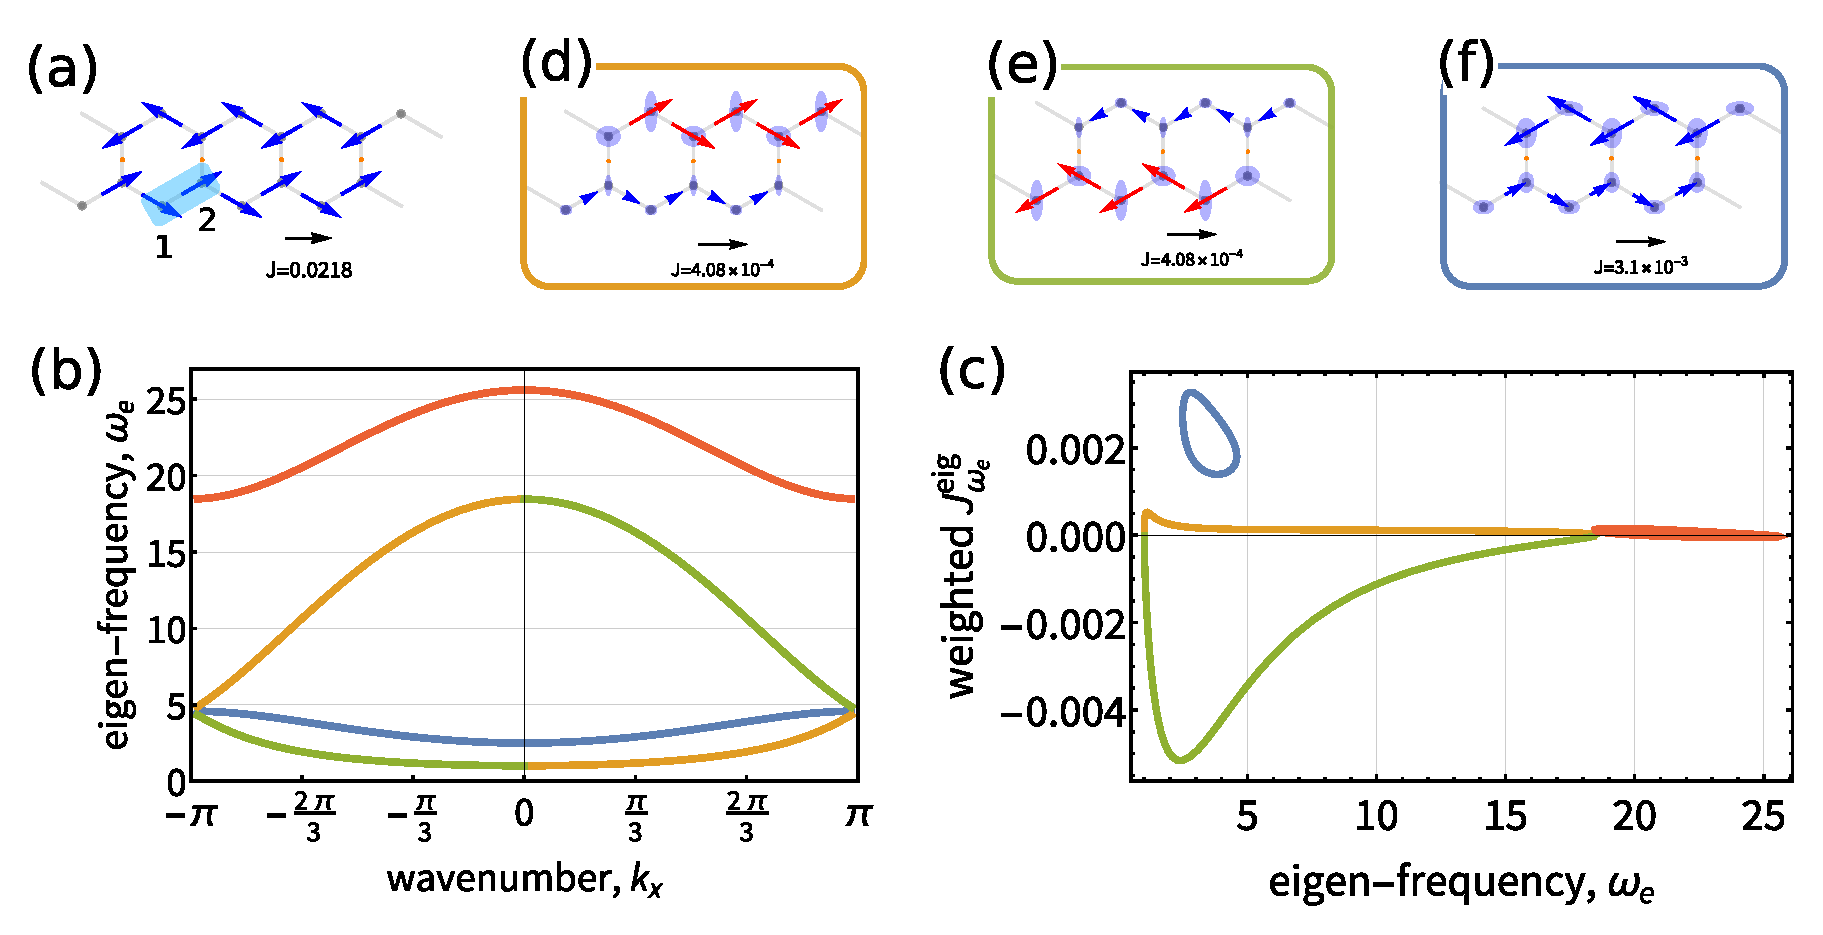
\includegraphics[width=0.8\textwidth]{eigen_modes.pdf}
    \caption{
        Using the eigenmode decomposition, we explain how the flux in honeycomb network is CCW, even though its edgemodes contribute to CW fluxes.
        (a) Network used for calculation, which consists of one row of hexagons (51 unit cells) and has periodic boundary in $x$ direction. Parameters: $k_{g,\tau}=1, k=10$, others are $1$.
        (b) Band structure of the network (marked with different colors). The yellow/green band contains CW flux localized on the top/bottom edge (an example mode is shown in (d)/(e)). The blue band contains bulk modes with CCW flux (also see (f)).
        (c) Weighted flux $J_{\omega_e}^{eig}$ from $1$ to $2$ (marked in (a)) of the four bands. Total flux in the green band with CW edge modes and the blue band with CCW bulk modes are $-0.106$ and $0.115$, respectively. As a result, the net flux is CCW.
    }
    \label{fig:eigen_modes}
\end{figure}

As an application, we will analyze the flux in the honeycomb network using the eigenmode decomposition \eqnname~\eqref{eqnS:flux_eigen} and the ``sum rule" \eqnname~\eqref{eqnS:eigen_sum_rule}.
The flux pattern in the active honeycomb network displays CCW flux localized on the boundary (\figurename~1b). This localization is reminiscent of the edgemode in \cite{Nash2015TopologicalMechanics} (\figurename~\ref{fig:Fourier_modes}b), however, their directions are opposite.
From the decomposition \eqnname~\eqref{eqnS:flux_eigen}, the edgemodes should contribute a large CW flux in the active system, but somewhat surprisingly, the net flux is CCW.
To better analyze the contribution from each eigenmode, we look at a simple honeycomb lattice with only one layer (\figurename~\ref{fig:eigen_modes}a).
This lattice has four bands (\figurename~\ref{fig:eigen_modes}b), two bulk bands (blue, red) and two edge bands (green, yellow). The weighted flux of each band is plotted in \figurename~\ref{fig:eigen_modes}c. We see that the CW edge band does contribute a large CW flux (green curve in \figurename~\ref{fig:eigen_modes}c), however, due to the ``sum rule", the unweighted sum of other bands has to be CCW. In the honeycomb lattice, it happens that many of this CCW fluxes are contained in the lower bulk band (blue curve in \figurename~\ref{fig:eigen_modes}c and example mode in \figurename~\ref{fig:eigen_modes}f). When the flux gets weighted, the CCW flux from lower bulk band outweighs CW flux from the edgemodes, the other two bands (yellow and red curve in \figurename~\ref{fig:eigen_modes}c) also contribute to CCW flux, although relatively small. As a result, the net flux is CCW, which is opposite to the flux of the edgemode.


\section{Derivation of eigenmode decomposition of energy flux}

To derive the eigenmode decomposition \eqnname~\eqref{eqnS:flux_eigen}, we first look at the reference isolated system, write down its eigenmodes \eqnname~\eqref{eqnS:mode_zct} and time-averaged energy flux \eqnname~\eqref{eqnS:mode_J_isolated}. Then we turn to the active system and decompose the flux \eqnname~\eqref{eqnS:flux_residue} using the eigenmodes to get \eqnname~\eqref{eqnS:mode_J_active}. Finally we show that the flux from these two sides are actually related in \eqnname~\eqref{eqnS:mode_J_relation}.
Lastly we also derive the ``sum rule" \eqnname~\eqref{eqnS:mode_J_sum}.

\subsection{Reference isolated system}
The reference isolated system has first-order gyroscopic dynamics as in \cite{Nash2015TopologicalMechanics}. In the setup with Lorentz force, the dynamical equation can be obtained by setting the mass to zero, and replacing the force matrix $K$ by ${K^\tau \equiv K + (\frac{\gamma}{\tau} + \frac{m}{\tau^2})I}$
\begin{equation}
    \dot{z} = \frac{1}{B} A K^\tau z.
\end{equation}
Following \cite{Nash2015TopologicalMechanics}, we convert to complex representation with $z^c \equiv \pmqty{x + iy & x - iy}^T$
\begin{equation}
i \dot{z}^c = \Omega z^c,\quad
K^\tau = i B A O^{-1} \Omega O
\end{equation}
where $O,O^{-1}$ are the transformations between $z$ and $z^c$ $z^c = Oz, z = O^{-1}z^c$.

Writing the eigenvalue problem as
\begin{equation}
\Omega u_{\omega_e} = \omega_e u_{\omega_e} ,
\end{equation}
the eigenmode with eigen-frequency $\omega_e$ reads
\begin{equation} \label{eqnS:mode_zct}
z^c_{\omega_e}(t) =  (u_{\omega_e} e^{-i\omega_e t} + u_{-\omega_e} e^{i\omega_e t})z_0 ,
\end{equation}
where $z_0$ is the amplitude, and it will be specified shortly.
The eigenmode needs a combination of $\omega_e$ and $-\omega_e$ to ensure that the motion of $x$ and $y$ is real-valued.
Mathematically, this combination is possible because of a symmetry in this eigenvalue problem, when there is $\omega_e$, there is also solution $-\omega_e$ with $u_{-\omega_e} = \pmqty{ 0 & I \\ I & 0 } u_{\omega_e}^*$.

A related property we need later is that, the left eigenvector $v_{\omega_e}$ can be expressed as $v_{\omega_e} = c_{\omega_e} \pmqty{ -I & 0 \\ 0 & I } u_{\omega_e}$,
where $c_{\omega_e}$ is a real prefactor to ensure normalization $v_{\omega_e}^T u_{\omega_e} = 1$.
If there are degenerate eigenvectors (like $v_{\omega_e}^{1},v_{\omega_e}^{2},\dots$), we choose an orthonormal basis set, i.e. $v_{\omega_e}^{i,T} u_{\omega_e}^{j} = 0$ for $i \neq j$.
With the introduction of $c_{\omega_e}$, we now set the amplitude $z_0$ to
$z_0^2 = -2 c_{\omega_e} T_a / \omega_e B$, such that the energy of the eigenmode is $T_a$.

The instantaneous energy flux $J_{\omega_e}$ of mode $z^c_{\omega_e}$ writes
\begin{equation}
\begin{split}
J_{\omega_e} &= (O^{-1} v^{c}_{\omega_e})^T A^J O^{-1}z^c_{\omega_e} \\
&= \tr O^{-1,T} A^J O^{-1}z^c_{\omega_e} v^{cT}_{\omega_e} .
\end{split}
\end{equation}
From the expression of mode \eqnname~\eqref{eqnS:mode_zct},
\begin{equation}
z^c_{\omega_e} v^{cT}_{\omega_e} = -i\omega_e(u_{\omega_e} e^{-i\omega_e t} + u_{-\omega_e}e^{i\omega_e t})(u_{\omega_e}^T e^{-i\omega_e t} - u_{-\omega_e}^Te^{i\omega_e t})z_0^2 .
\end{equation}
When averaging over time, terms like $e^{\pm 2i\omega_e t}$ vanish, so we get
\begin{equation}
\overline{z^c_{\omega_e} v^{cT}_{\omega_e}} = i\omega_e(u_{\omega_e} u_{-\omega_e}^T - u_{-\omega_e} u_{\omega_e}^T)z_0^2 .
\end{equation}
Plugging in $z_0^2 = -2 c_{\omega_e} T_a / \omega_e B$, the time-averaged flux of the eigenmode $J_{\omega_e}^\text{eig}$ reads
\begin{equation} \label{eqnS:mode_J_isolated}
J_{\omega_e}^\text{eig} = -\frac{2T_ak}{B} ic_{\omega_e} \tr O^{-1,T}A^JO^{-1} (u_{\omega_e} u_{-\omega_e}^T - u_{-\omega_e} u_{\omega_e}^T) .
\end{equation}

\subsection{Active system}
Now we turn to the active system, and the starting point is \eqnname~\eqref{eqnS:flux_residue}.
We need to decompose $G^\tau \equiv G^+(-i/\tau)$ into modes as below,
\begin{align}
G^\tau &= \frac{i}{B} O^{-1} (\Omega - \frac{i}{\tau}I)^{-1} OA ,\\
(\Omega - \frac{i}{\tau}I)^{-1} &=
\sum_{\omega_e > 0}\frac{i\tau}{1 + \omega_e^2 \tau^2}  (u_{\omega_e} v_{\omega_e}^T + u_{-\omega_e} v_{-\omega_e}^T) + \\
&\quad \sum_{\omega_e > 0}\frac{\omega_e\tau^2}{1 + \omega_e^2 \tau^2}  (u_{\omega_e} v_{\omega_e}^T - u_{-\omega_e} v_{-\omega_e}^T) ,\\
G^\tau &= \sum_{\omega_e > 0}\frac{-\tau/B}{1 + \omega_e^2 \tau^2} O^{-1} (u_{\omega_e} v_{\omega_e}^T + u_{-\omega_e} v_{-\omega_e}^T) OA + \\
&\quad \sum_{\omega_e > 0}\frac{i\omega_e\tau^2/B}{1 + \omega_e^2 \tau^2} O^{-1} (u_{\omega_e} v_{\omega_e}^T - u_{-\omega_e} v_{-\omega_e}^T) OA .
\end{align}
The averaged flux $\expval{J}$ reads
\begin{equation}
\begin{split}
\expval{J} &=
\sum_{\omega_e > 0}\frac{T_ak/(2B)}{1 + \omega_e^2 \tau^2} \tr O^{-1} (u_{\omega_e} v_{\omega_e}^T + u_{-\omega_e} v_{-\omega_e}^T) OAA^{as} + \\
&\quad \sum_{\omega_e > 0}\frac{-i\omega_e T_ak\tau/(2B)}{1 + \omega_e^2 \tau^2} \tr O^{-1} (u_{\omega_e} v_{\omega_e}^T - u_{-\omega_e} v_{-\omega_e}^T) OAA^{as}.
\end{split}
\end{equation}
The second term can be shown to be zero,
$\tr OAA^{as}O^{-1} (u_{\omega_e} v_{\omega_e}^T - u_{-\omega_e} v_{-\omega_e}^T) = 0$.
So the mode decomposition in its preliminary form reads
\begin{gather}
\expval{J} = \sum_{\omega_e} \expval{J}_{\omega_e} ,\\
\expval{J}_{\omega_e} \equiv \frac{T_ak}{2B}\frac{1}{1 + \omega_e^2 \tau^2} \tr OAA^{as}O^{-1} (u_{\omega_e} v_{\omega_e}^T + u_{-\omega_e} v_{-\omega_e}^T). \label{eqnS:mode_J_active}
\end{gather}

\subsection{The relationship between isolated system and active system}
Now we need to find relationship between these two fluxes $\expval{J}_{\omega_e}$ \eqnname~\eqref{eqnS:mode_J_active} and $J_{\omega_e}^\text{eig}$ \eqnname~\eqref{eqnS:mode_J_isolated}.
We will write $J_{\omega_e}^\text{eig}$ in a form that looks similar to
$\langle J\rangle_{\omega_e}$.
Converting $A^{J}$ to $A^{as}$ using $A^{as}=-(A_J-A_J^T)$, and $u_{\omega_e}$ to $v_{\omega_e}$ using $v_{\omega_e} = c_{\omega_e} \pmqty{ -I & 0 \\ 0 & I } u_{\omega_e}$, we get
\begin{equation}
J_{\omega_e}^\text{eig} = -\frac{iT_ak}{B} \tr AO^{-1,T}A^{as}O^{-1} (u_{\omega_e} v_{\omega_e}^T + u_{-{\omega_e}}v_{-{\omega_e}}^T) .
\end{equation}
From direct calculation, $AO^{-1,T} = \frac{i}{2} OA$, and $J_{\omega_e}^\text{eig}$ becomes the same as $\expval{J}_{\omega_e}$ apart from a factor
\begin{equation} \label{eqnS:mode_J_isolated_mod}
J_{\omega_e}^\text{eig} = \frac{T_ak}{2B} \tr OAA^{as}O^{-1} (u_{\omega_e} v_{\omega_e}^T + u_{-{\omega_e}}v_{-{\omega_e}}^T) .
\end{equation}

Comparing \eqnname~\eqref{eqnS:mode_J_isolated_mod} with \eqref{eqnS:mode_J_active}, we derived the relationship between flux from active system and isolated system
\begin{equation} \label{eqnS:mode_J_relation}
\expval{J}_{\omega_e} = \frac{1}{1 + {\omega_e}^2 \tau^2} J_{\omega_e}^\text{eig} .
\end{equation}

Lastly, we show that the unweighted sum of $J_{\omega_e}^\text{eig}$ is zero.
This unweighted sum reads
\begin{equation}
\sum_{\omega_e} J_{\omega_e}^\text{eig} = \frac{T_ak}{2B} \tr [O A A^{as} O^{-1} UV^T],
\end{equation}
where $U$ is the collection of all right eigenvectors $U = \pmqty{u_{\omega_e,1} & u_{\omega_e,2} & \cdots}$, and likewise for $V$.
Since $UV^T = I$ from orthonormality, this sum vanishes
\begin{equation} \label{eqnS:mode_J_sum}
\sum_{\omega_e} J_{\omega_e}^\text{eig} = \frac{T_ak}{2B} \tr A A^{as} = 0.
\end{equation}


\section{Path summation of energy flux}
To derive the path summation formula \eqnname~(11) and the path rules, we start from \eqnname~\eqref{eqnS:flux_residue}, expand around a noninteracting reference system with $k=0$ to get \eqnname~\eqref{eqnS:smallk_expand}, discuss the convergence radius in \eqnname~\eqref{eqnS:smallk_convergence}, then insert resolution of identity to make each term representable by a path as in \eqnname~\eqref{eqnS:smallk_Sl}, and arrive at the path summation formula in \eqref{eqnS:smallk_path_sum}.
We also provide a convenient way to calculate $S_{-l}$ in \eqnname~\eqref{eqnS:smallk_S-l}, and a heuristic interpretation of $S_l$ in \eqnname~\eqref{eqnS:smallk_path_vector}.

\subsection{Derivation of path summation formula}
Similar to the last section, the central object is $G^\tau$.
In the noninteracting case ($k=0$), $G^\tau$ is analytically solvable. We denote $G^\tau(k=0) = G^\tau_0$.
The inverse $(G^\tau_0)^{-1}$ has a block diagonal form,
\begin{equation}
    (G^\tau_0)^{-1} = k_{g,\tau} I + \frac{B}{\tau}A
    = \sum_i \ketbra{i}{i} \otimes (k_{g,\tau}I + \frac{B}{\tau} \pmqty{0 & 1 \\ -1 & 0}).
\end{equation}
where $k_{g,\tau} \equiv k_g + \frac{\gamma}{\tau} + \frac{m}{\tau^2}$.
Then $G^\tau_0$ is also block diagonal, with each block the inverse of the blocks above,
\begin{equation} \label{eqnS:smallk_Gtau0}
    G^\tau_0 = \sum_i \ketbra{i}{i} \otimes \frac{1}{(k_{g,\tau})^2 + (B/\tau)^2}(k_{g,\tau} I - \frac{B}{\tau} \pmqty{0 & 1 \\ -1 & 0})
    = \sum_i \ketbra{i}{i} \otimes \frac{1}{k_0}R_\alpha,
\end{equation}
where $k_0 \equiv \sqrt{(k_{g,\tau})^2 + (B/\tau)^2}$, and $R_\alpha$ is the rotation matrix with angle $\alpha \equiv \arcsin{\frac{B/\tau}{k_0}}$, $R_\alpha = \pmqty{\cos\alpha & -\sin\alpha \\ \sin\alpha & \cos\alpha}$.

We now turn on $k$. We denote the inter-particle part of the force matrix $K$ as $k K_s$, where the factor $k$ is extracted so that the matrix $K_s$ is dimensionless. The blocks of $K_s$ read
\begin{equation} \label{eqnS:smallk_matKs}
    \mel{i}{K_s}{i} = \sum_{i'} e_{ii'}e_{ii'}^T, \quad
    \mel{i}{K_s}{j} = e_{ij}e_{ji}^T.
\end{equation}
Then $G^\tau$ reads
\begin{equation}
    G^\tau = \frac{1}{(G^\tau_0)^{-1} + k K_s}
    = \frac{1}{k_0} [(k_0 G^\tau_0)^{-1} + \frac{k}{k_0}K_s]^{-1}
\end{equation}
In small $k/k_0$ regime, this matrix inversion can be expanded as
\begin{equation} \label{eqnS:smallk_expand}
    \begin{split}
    G^\tau &= \frac{1}{k_0} [(k_0 G^\tau_0) + \frac{k}{k_0} (k_0 G^\tau_0) (-K_s) (k_0 G^\tau_0) + (\frac{k}{k_0})^2 (k_0 G^\tau_0) (-K_s) (k_0 G^\tau_0) (-K_s) (k_0 G^\tau_0) + \dots ]\\
    &= \frac{1}{k_0} (k_0 G^\tau_0) \sum_{n=0}^{\infty}[\frac{k}{k_0}(-K_s)(k_0 G^\tau_0)]^n.
    \end{split}
\end{equation}
To find the convergence radius, we can write the eigen-decomposition of the matrix $(-K_s)(k_0 G^\tau_0)$ as $(-K_s)(k_0 G^\tau_0) = W\Lambda W^{-1}$, where $\Lambda$ is the diagonal matrix that contains all eigenvalues $\lambda_i$'s, then the flux becomes
\begin{equation}
    \begin{split}
    \expval{J} &\propto \tr G^\tau A^{as}
    \propto \sum_{n=0}^{\infty}\tr (k_0 G^\tau_0) [\frac{k}{k_0}W\Lambda W^{-1}]^n A^{as} \\
    &= \sum_i [W^{-1} A^{as} (k_0 G^\tau_0) W]_{ii} \sum_n (\frac{k}{k_0} \lambda_i)^n.
    \end{split}
\end{equation}
For terms in the series to be convergent, $\frac{k}{k_0}$ should satisfy
\begin{equation} \label{eqnS:smallk_convergence}
    \frac{k}{k_0} < \frac{1}{\max_i\abs{\lambda_i}}.
\end{equation}

Before inserting resolution of identity to make paths, we note that the matrix $A^{as}$ and $K_s$ have common blocks, $A^{as} = -\ket{i}\bra{j} \otimes e_{ij}e_{ji}^T + \ket{j}\bra{i} \otimes e_{ji}e_{ij}^T$ and $\mel{i}{K_s}{j} = e_{ij}e_{ji}^T$, so that $A^{as}$ can merge with the series of $G^\tau$.
\begin{equation} \label{eqnS:smallk_J_block}
    \begin{split}
    \frac{\expval{J}}{T_a/\tau} = -\frac{k}{2} (\tr G^\tau A^{as})
    &= -\frac{k}{2} (\tr \mel{i}{G^\tau}{j} e_{ji}e_{ij}^T - \tr \mel{j}{G^\tau}{i} e_{ij}e_{ji}^T) \\
    &= \frac{k}{2} (\tr \mel{i}{G^\tau}{j} \mel{j}{-K_s}{i} - \tr \mel{j}{G^\tau}{i} \mel{i}{-K_s}{j}).
    \end{split}
\end{equation}

Now we use the expansion \eqnname~\eqref{eqnS:smallk_expand}, and look at the contribution of its $(n-1)$'th-order term to the first term of the flux, $k \tr \mel{i}{\frac{1}{k_0} (k_0 G^\tau_0) [\frac{k}{k_0}(-K_s)(k_0 G^\tau_0)]^{n-1}}{j} \mel{j}{-K_s}{i}$.
If $n-1=0$, this term vanishes, so we only need to consider $n-1 \ge 1$ case.
Insert $n-1$ resolution of identity $I = \sum_{l_a=1}^N \ketbra{l_a}{l_a}$, and plug in $k_0 G^\tau_0$ \eqnname~\eqref{eqnS:smallk_Gtau0} and $K_s$ \eqnname~\eqref{eqnS:smallk_matKs}, we get
\begin{equation}
    \begin{split}
    &\frac{k}{k_0} \tr \mel{i}{(k_0 G^\tau_0) [\frac{k}{k_0}(-K_s)(k_0 G^\tau_0)]^{n-1}}{j} \mel{j}{-K_s}{i} \\
    =& (\frac{k}{k_0})^n \sum_{l_1,l_2,\dots,l_{n-1}} \tr \bra{i} (k_0G^\tau_0) \ket{l_{n-1}}\bra{l_{n-1}} (-K_s) (k_0G^\tau_0) \cdots \ket{l_1}\bra{l_1} (-K_s) (k_0G^\tau_0) \ket{j} \mel{j}{-K_s}{i}\\
    =& (\frac{k}{k_0})^n \sum_{l_1,l_2,\dots,l_{n-2}} \tr R_\alpha (-K_s)_{il_{n-2}} R_\alpha \cdots (-K_s)_{l_1j} R_\alpha (-K_s)_{ji},
    \end{split}
\end{equation}
where $(-K_s)_{l_bl_a} \equiv \mel{l_b}{-K_s}{l_a}$.
We will denote path $l = i\rightarrow j\rightarrow l_1\rightarrow l_2\rightarrow \dots \rightarrow l_{n-2}\rightarrow i$, and its corresponding term in the above summation as $S_l$
\begin{equation} \label{eqnS:smallk_Sl}
    S_l = (\frac{k}{k_0})^n \tr R_\alpha (-K_s)_{il_{n-2}} R_\alpha \cdots (-K_s)_{l_1j} R_\alpha (-K_s)_{ji}.
\end{equation}

The second term of the flux in \eqref{eqnS:smallk_J_block} can be treated similarly, and it results in $S_{-l}$, where $-l$ means path $l$ in its reversed order.
Combining \eqnname~\eqref{eqnS:smallk_Sl} and \eqref{eqnS:smallk_J_block}, we get the path summation formula of the flux
\begin{equation} \label{eqnS:smallk_path_sum}
    \frac{\expval{J}}{T_a/\tau} = \sum_l J^\text{path}_l
    = \sum_l \frac{1}{2}(S_l - S_{-l}).
\end{equation}

\subsection{Path rules and discussions}
The path rules can be extracted from the expression of $S_l$ and $J^\text{path}$.
From the element $(-K)_{l_bl_a}$ in $S_l$, we see that either $l_a,l_b$ are bonded, or $l_a=l_b$, otherwise $(-K)_{l_bl_a}=0$.
So the path has to be a closed walk along the edges of the network.
From $J^\text{path}_l$ for flux from $i$ to $j$, we see that if the path contains equal numbers of $i\rightarrow j$ and $j\rightarrow i$, the net contribution is zero. Because, either $l=-l$, so $J^\text{path}_l \propto S_l - S_{-l} = 0$, or $l'\equiv -l$ is another path, and $J^\text{path}_l + J^\text{path}_{l'} = 0$.

To calculate $S_{-l}$, there is a convenient way given that $S_l$ is known.
Based on the transformation below, $S_{-l}$ can be obtained by taking the result of $S_l$, then replacing $\alpha$ by $-\alpha$.
\begin{equation} \label{eqnS:smallk_S-l}
    \begin{split}
    S_{-l} / (\frac{k}{k_0})^n
    &= \tr (R_\alpha (-K_s)_{ij} R_\alpha (-K_s)_{jl_1} \cdots R_\alpha  (-K_s)_{l_{n-2}i})^T \\
    &= \tr (-K_s)_{l_{n-2}i}^T R_\alpha^T \cdots (-K_s)_{jl_1}^T R_\alpha^T (-K_s)_{ij}^T R_\alpha^T \\
    &= \tr R_{-\alpha} (-K_s)_{il_{n-2}} R_{-\alpha} \cdots (-K_s)_{l_1j} R_{-\alpha} (-K_s)_{ji}.
    \end{split}
\end{equation}

To interpret $S_l$ in a more heuristic way, we insert $I = e_{ij}e_{ij}^T + e_{ij,\perp}e_{ij,\perp}^T$ to the trace in \eqnname~\eqref{eqnS:smallk_Sl}, where $e_{ij,\perp}$ denotes the unit direction perpendicular to $e_{ij}$.
Because $(-K_s)_{ji}e_{ij,\perp} = 0$, the trace reduces to a matrix product
\begin{equation} \label{eqnS:smallk_path_vector}
    S_l/(\frac{k}{k_0})^n = e_{ij}^T R_\alpha (-K_s)_{i l_{n-2}} R_\alpha \cdots (-K_s)_{l_1j} R_\alpha (-K_s)_{ji} e_{ij}.
\end{equation}
This expression means the following operations:
starting from a unit displacement of $i$ along $e_{ij}$, $j$ would be displaced according to the force $(-K_s)_{ji} e_{ij}$, after which $j$ is rotated by angle $\alpha$; then start from $j$ and perform similar operations for $(-K_s)_{l_1j}$ and $R_\alpha$; finally, the transmission goes back to $i$; we project the displacement onto $e_{ij}$, and this value is $S_l$ (apart from the prefactor $(\frac{k}{k_0})^n$).

\subsection{Flux of polygon paths}
Here we write down the flux formula for a polygon path without loops.
It is easier to work in local coordinates, where each node has its own coordinate system.
For node $i$ in the path, let the outer angle from $i$ to $i-1$ be $\pi$, and the angle from $i$ to $i+1$ be $\theta_i$.
Then the matrix $(-K_s)_{i+1,i}$ reads
\begin{equation}
    (-K_s)_{i+1,i}
    = -e_{i+1,i} e_{i,i+1}^T
    = -\pmqty{-1 \\ 0} \pmqty{\cos\theta_i & \sin\theta_i}
    = \pmqty{1 \\ 0} \pmqty{\cos\theta_i & \sin\theta_i}.
\end{equation}
The trace in $S_l$ becomes
\begin{equation}
    \begin{split}
    S_l / (\frac{k}{k_0})^n
    &= \tr \prod_i (-K_s)_{i+1,i} R_\alpha
    = \tr \prod_i \pmqty{1 \\ 0} \pmqty{\cos\theta_i & \sin\theta_i} R_\alpha \\
    &= \prod_i \pmqty{\cos\theta_i & \sin\theta_i} R_\alpha \pmqty{1 \\ 0}
    = \prod_i \cos(\theta_i - \alpha)
    \end{split}
\end{equation}
So the flux for this path without loops writes
\begin{equation} \label{eqnS:smallk_path_polygon}
    J^\text{path}_\text{polygon} = \frac{1}{2} (\frac{k}{k_0})^n (\prod_i \cos(\theta_i - \alpha) - \prod_i \cos(\theta_i + \alpha)).
\end{equation}

\subsection{Contribution from higher-order paths}
\begin{figure}[tbp]
	\centering
	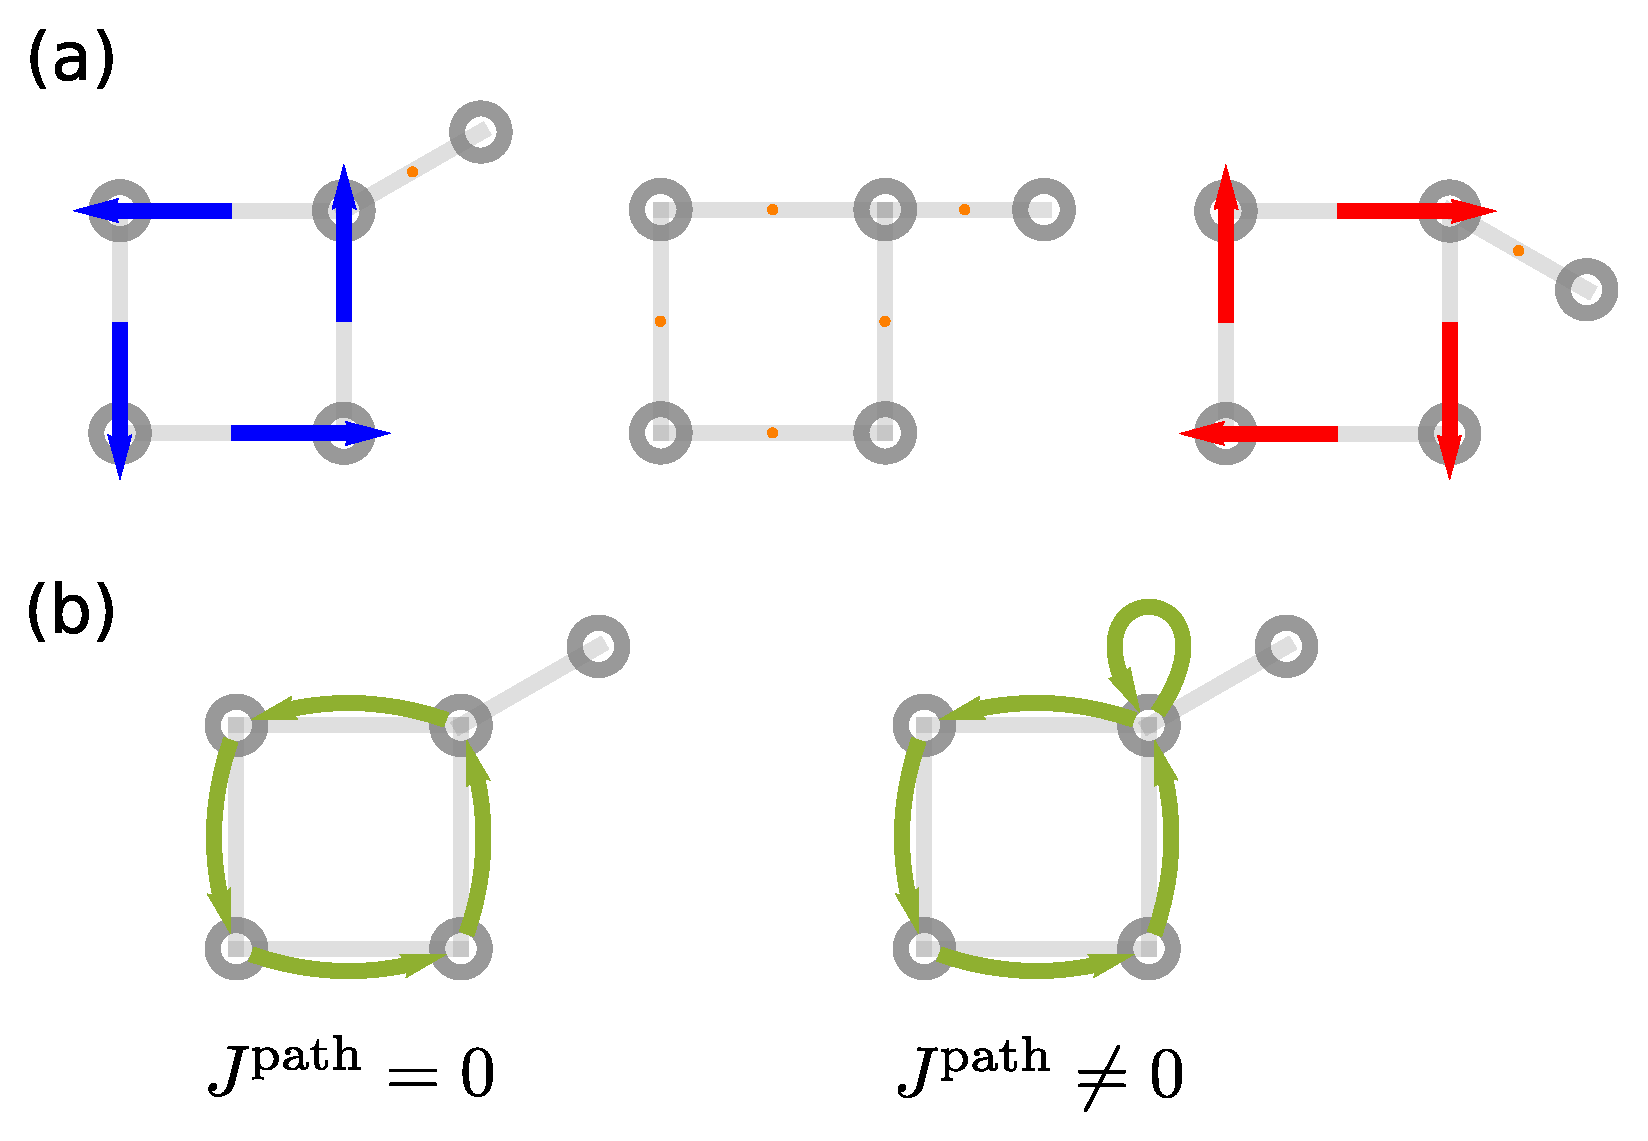
\includegraphics[width=0.5\textwidth]{path_square_tail.pdf}
    \caption{
        Higher-order paths in a tailed-square network.
        (a) Direction of flux can be controlled by the orientation of the side-chain.
        (b) From diagrammatic approach, the flux of the lowest-order path (square) vanishes, and the first non-vanishing path is affected by the side-chain.
    }
    \label{fig:path_square_tail}
\end{figure}

\begin{figure}[tbp]
	\centering
	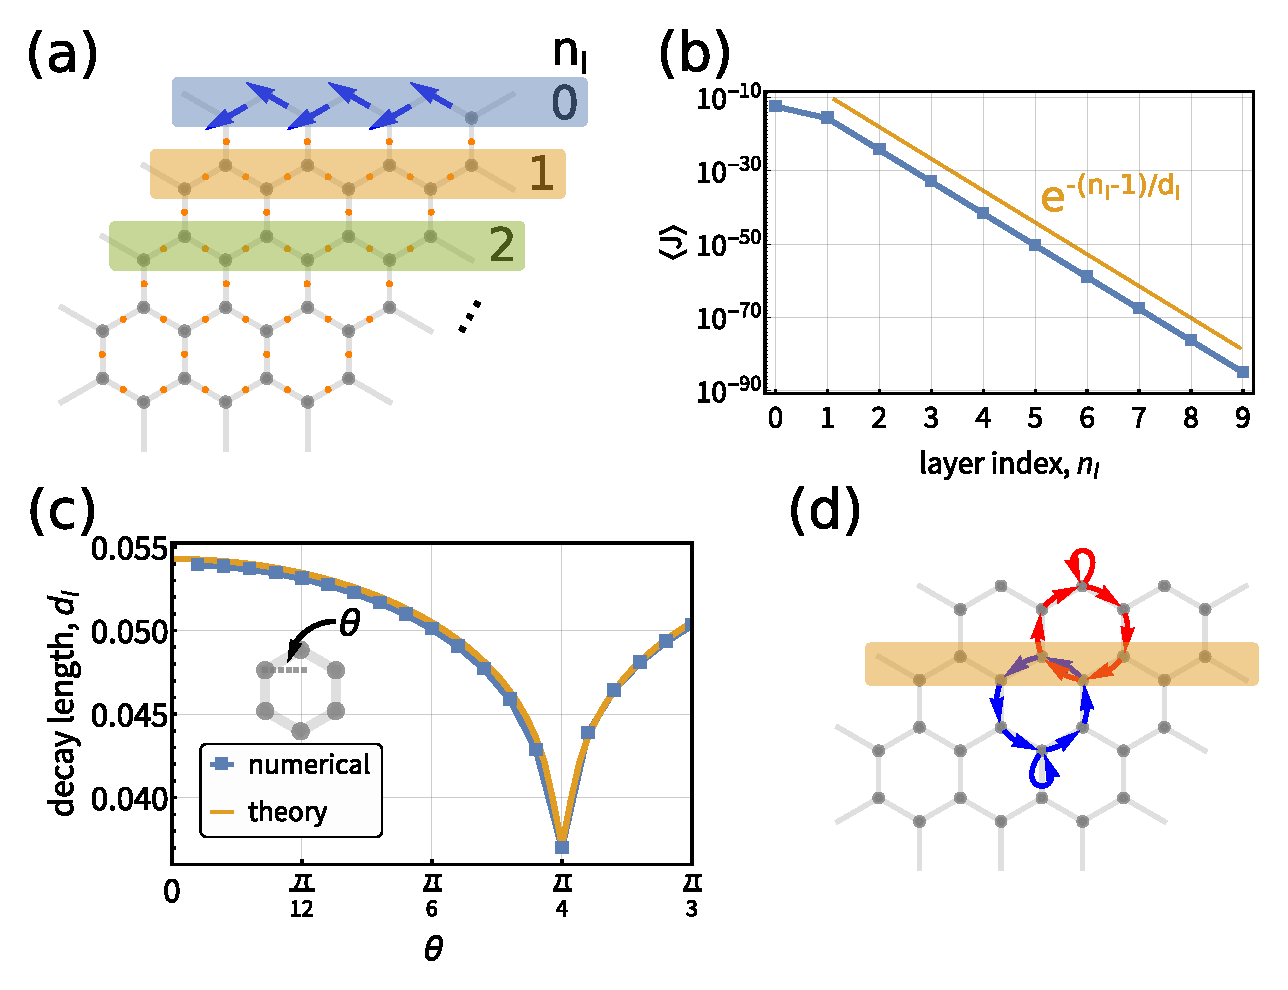
\includegraphics[width=0.6\textwidth]{path_decay.pdf}
    \caption{
        Decay of fluxes away from the boundary of honeycomb networks, and explanation using the diagrammatic technique.
        (a) Schematic of a honeycomb network which is periodic in the $x$ direction. Layers from the boundary are indexed as $n_l$.
        (b) Semi-log plot of flux $\expval{J}$ at layer $n_l$. The flux starting from layer $n_l=1$ shows exponential decay, with decay length $d_l$. Parameters used for numerical calculations are $\theta = \pi/6, k/k_0 = 0.01, \alpha = \pi/4$.
        (c) Decay length $d_l$ changes with the network angle $\theta$ non-monotonically, and the curve has a cusp at $\theta = \alpha = \pi/4$. At small $k/k_0$, perturbation theory results agree with numerical calculations.
        (d) The first non-vanishing path pair for $n_l=1$ has length $7$. The two paths do not cancel, because the loop in the bulk and at the boundary have different values.
    }
    \label{fig:path_decay}
\end{figure}

In some situations, the contribution of polygonal paths vanish, and higher order paths with loops become dominant. Unlike in polygonal paths, paths with loops are affected by side-chains.

One situation is when the polygon path itself vanishes. In \figurename~\ref{fig:path_square_tail}a, the flux of lowest order path, square (\figurename~\ref{fig:path_square_tail}b), is zero, so the main contribution comes from the path with length $5$ (\figurename~\ref{fig:path_square_tail}b). Through the loop in this path, the orientation of the side-chain controls the flux direction in the main square, without changing the geometry of the main cycle (as seen in \figurename~1b).

Another situation is that two polygon paths cancel each other, which happens in honeycomb-like networks away from the boundary (\figurename~\ref{fig:path_decay}a).
With careful calculations, the fluxes for $n_l\ge 1$ are not zero, they rather appear as an exponential decay (\figurename~\ref{fig:path_decay}b). By changing the geometric angle $\theta$, the decay length varies non-monotonically, and has a cusp at $\theta=\alpha$ (\figurename~\ref{fig:path_decay}c).
This decay and its relationship with $\theta$ can be explained by considering the paths.
While the hexagon path constitutes the lowest-order path at the boundary, it vanishes for $n_l\ge 1$ due to cancellations. The first non-vanishing pair of paths for $n_l=1$ is shown in \figurename~\ref{fig:path_decay}d, in which the loop exploits the asymmetry between the bulk side (with a vertical bond at the blue loop) and the boundary side (with no vertical bonds at the red loop). For every increment of one layer, the length of paths increases by $4$. So the flux at layer $n_l$ is on the order of $k^{4n_l+3}$, which exhibits an exponential decay $e^{-(n_l-1)/d_l}$.
Through the calculation of these paths, we get the decay length $d_l = -1/\log[4(k/k_0)^4(\sin(\theta+\alpha)\sin(\theta-\alpha))^2]$. From this result, we see that the cusp at $\theta=\alpha$ in \figurename~\ref{fig:path_decay}c is due to the term $\sin(\theta-\alpha)$. In fact, at the special point $\theta=\alpha$, paths like \figurename~\ref{fig:path_decay}d vanish, and we need to consider even higher-order paths.


\section{Simulation of active gyroscopic network coupled with a passive segment}
A simulation is shown in the Supplemental Video, which presents both the motion of particles and the energy flux through the color-labelled bonds.
The energy fluxes are in general random. During the period when $J$ is large, $J$ shows successive peaks, indicating a large energy flow from left to right. The spacing between the peaks matches the sound speed of the elastic chain ($\sqrt{k/m}$). Although the averaged direction of energy flux is from left to right, the instantaneous flux can also transport from right to left, shown as negative peaks. 

The simulation is performed using LAMMPS \cite{Plimpton1995FastParallel} with Moltemplate toolkit \cite{Jewett2013MoltemplateCoarseGrained} and custom code.
We used a Trotter splitting method \cite{Tuckerman1992ReversibleMultiple,Bussi2007AccurateSampling} to simulate the underdamped Langevin dynamics.
The integrator combines the integrator for colored noise \cite{Ceriotti2010ColoredNoiseThermostats} and that for Lorentz force \cite{Chin2008SymplecticEnergyconserving}.
We did not simulate the commonly-used overdamped Langevin dynamics, because some intricacy arises when the system also experiences a Lorentz force \cite{Chun2018EmergenceNonwhite}.
Below, we first define each step in the integrator, then present the combined result.

The velocity-Verlet step $U_{vv}$ is the integrator when both Lorentz force and the colored noise are absent. It is defined as
\begin{align}
U_{vv}(\Delta t):\quad
&v \leftarrow v + F(x) \Delta t / (2m) \\
&x \leftarrow x + v \Delta t \\
&v \leftarrow v + F(x) \Delta t / (2m),
\end{align}
where $F(x)$ is the conservative force, including on-site and inter-particle potentials.

Writing the Lorentz force part as
\begin{equation}
\dot{v} = -\pmqty{ 0 & B/m \\ -B/m & 0 } \pmqty{ v_x \\ v_y }
\equiv -a_p v ,
\end{equation}
then its integrator $U_L$ is a rotation of the velocity
\begin{equation}
    U_{L}(\Delta t):\quad
    v \leftarrow e^{-\Delta t a_p} v .
\end{equation}

Writing the colored noise part as
\begin{gather}
    \frac{d}{dt} \pmqty{ v \\ \eta }
    = -A_p \pmqty{ v \\ \eta } + B_p \pmqty{ \xi_w \\ \xi_a }, \\
    A_p = \pmqty{ \frac{\gamma}{m} & -\frac{1}{m} \\ 0 & \frac{1}{\tau} },\quad
    B_p = \pmqty{ 0 & 0 \\ 0 & \frac{\sqrt{2\gamma T_a}}{\tau} },
\end{gather}
then its integrator $U_{OUP}$ reads
\begin{equation}
    U_{OUP}(\Delta t):\quad
    \pmqty{ v \\ \eta } \leftarrow T(\Delta t) \pmqty{ v \\ \eta } + S(\Delta t) \pmqty{ 0 \\ N_a },
\end{equation}
where $N_a$ is the standard Gaussian random variable, and
\begin{align}
T(\Delta t) &= e^{-\Delta t A_p} ,\\
S(\Delta t)S(\Delta t)^T &= C_p - T(\Delta t) C_p T(\Delta t) ^T .
\end{align}
$C_p$ is the solution of $A_p C_p + C_p A_p^T = B_pB_p^T$.
$S(\Delta t)$ can be solved as an upper-triangle matrix.

Combining these steps together, the integrator for one time step $\Delta t$ reads
\begin{equation}
    U(\Delta t) = U_{OUP}(\frac{\Delta t}{2})U_{L}(\frac{\Delta t}{2})U_{vv}(\Delta t)U_{L}(\frac{\Delta t}{2})U_{OUP}(\frac{\Delta t}{2}),
\end{equation}
where the order of operations is right-to-left.


\section{Relationship between swimmer's speed and energy flux}
To understand the proportionality between $V_s$ and $\expval{J}$, we turn to the diagrammatic technique. Different from previous cases, this path sum can be computed exactly, so the result holds beyond small $k$ regime.

First we rewrite $V_s$ as the following
\begin{equation}
    \frac{V_s}{7a/24L^2} = \expval{J_{12}^s} + \expval{J_{23}^s} + \expval{J_{31}^s}, \label{eqnS:swimmer_Vs}
\end{equation}
where we have defined $\expval{J_{ij}^s} \equiv \expval{(x_i-x_j)(v_i+v_j)}$. $\expval{J_{ij}^s}$ is proportional to the energy flux via $\expval{J_{ij}} = \frac{k_{ij}}{2}\expval{J_{ij}^s}$, where $k_{12}=k_{23}=k$, and $k_{31}=0$ (because $\expval{J_{31}} = 0$, there is no energy flux from $3$ to $1$).
We see that both $\expval{J_{12}^s}$ and $\expval{J_{23}^s}$ are proportional to the flux $\expval{J}$ apart from a factor $k$, so the remaining task is to find the relationship between $\expval{J_{31}^s}$ and $\expval{J}$ or $\expval{J_{12}^s}$.

\begin{figure}[tbp]
	\centering
	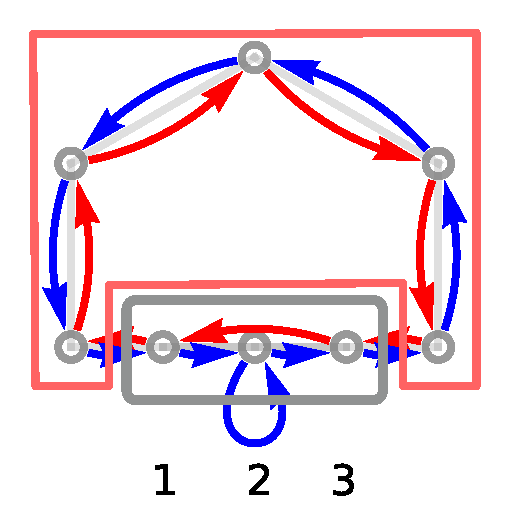
\includegraphics[width=0.4\textwidth]{swimmer_path.pdf}
    \caption{
        One example of $J_{31}^s$ path (red) and $J_{12}^s$ path (blue). Passive particles are boxed in gray, and the active ones are boxed in red.
    }
    \label{fig:swimmer_path}
\end{figure}

We use a diagrammatic technique with the modification that the paths should contain only one $3\rightarrow 1$ segment. This modification is a consequence of the fact that particle $3$ and $1$ are not bonded.
We now illustrate the correspondence between the paths for $\expval{J_{31}^s}$ and for $\expval{J_{12}^s}$. For each path $l$ for $\expval{J_{31}^s}$, we can construct $n$ paths for $\expval{J_{12}^s}$ by reversing $l$ then replacing $1\rightarrow 3$ by $1\rightarrow 2(\rightarrow 2)^n \rightarrow 3$, where $n=0,1,\dots$. An example construction of paths is shown in \figurename~\ref{fig:swimmer_path}.
For $\expval{J_{12}^s}$, all its paths can be constructed in this way.
As a result, there is a $1$ to $n$ correspondence between the paths for $\expval{J_{31}^s}$ and for $\expval{J_{12}^s}$, which leads to the relationship
\begin{equation}
    \expval{J_{12}^s} = \frac{k}{k_0}\sum_{n=0}^\infty (-2\frac{k}{k_0})^n (-\expval{J_{31}^s}) = \frac{k/k_0}{1-(-2k/k_0)} (-\expval{J_{31}^s}), \label{eqnS:swimmer_path_mapping}
\end{equation}
where $k_0 = k_g + m/\tau^2$ ($B,\gamma=0$ for the passive part), and the factor $-2\frac{k}{k_0}$ comes from the loop $2\rightarrow 2$.
Plugging \eqnname~\eqref{eqnS:swimmer_path_mapping} to the expression of $V_s$ \eqnname~\eqref{eqnS:swimmer_Vs}, we obtain the proportionality
\begin{equation}
    \frac{V_s}{7a/24L^2} = -\frac{k_0}{k} \frac{\expval{J}}{k/2},
\end{equation}
which is \eqnname~(15) in the main text.
Since we have considered all the paths, this result can be analytically continued to arbitrarily large $k$.

From this diagrammatic technique we also see that, the proportionality constant is independent of the geometry of the active part of the network. This is because the paths through the active part for $\expval{J_{31}^s}$ and for $\expval{J_{12}^s}$ are identical.


% \bibliography{reference}
%merlin.mbs apsrev4-1.bst 2010-07-25 4.21a (PWD, AO, DPC) hacked
%Control: key (0)
%Control: author (0) dotless jnrlst
%Control: editor formatted (1) identically to author
%Control: production of article title (0) allowed
%Control: page (1) range
%Control: year (0) verbatim
%Control: production of eprint (0) enabled
\begin{thebibliography}{14}%
\makeatletter
\providecommand \@ifxundefined [1]{%
    \@ifx{#1\undefined}
}%
\providecommand \@ifnum [1]{%
    \ifnum #1\expandafter \@firstoftwo
    \else \expandafter \@secondoftwo
    \fi
}%
\providecommand \@ifx [1]{%
    \ifx #1\expandafter \@firstoftwo
    \else \expandafter \@secondoftwo
    \fi
}%
\providecommand \natexlab [1]{#1}%
\providecommand \enquote  [1]{``#1''}%
\providecommand \bibnamefont  [1]{#1}%
\providecommand \bibfnamefont [1]{#1}%
\providecommand \citenamefont [1]{#1}%
\providecommand \href@noop [0]{\@secondoftwo}%
\providecommand \href [0]{\begingroup \@sanitize@url \@href}%
\providecommand \@href[1]{\@@startlink{#1}\@@href}%
\providecommand \@@href[1]{\endgroup#1\@@endlink}%
\providecommand \@sanitize@url [0]{\catcode `\\12\catcode `\$12\catcode
    `\&12\catcode `\#12\catcode `\^12\catcode `\_12\catcode `\%12\relax}%
\providecommand \@@startlink[1]{}%
\providecommand \@@endlink[0]{}%
\providecommand \url  [0]{\begingroup\@sanitize@url \@url }%
\providecommand \@url [1]{\endgroup\@href {#1}{\urlprefix }}%
\providecommand \urlprefix  [0]{URL }%
\providecommand \Eprint [0]{\href }%
\providecommand \doibase [0]{http://dx.doi.org/}%
\providecommand \selectlanguage [0]{\@gobble}%
\providecommand \bibinfo  [0]{\@secondoftwo}%
\providecommand \bibfield  [0]{\@secondoftwo}%
\providecommand \translation [1]{[#1]}%
\providecommand \BibitemOpen [0]{}%
\providecommand \bibitemStop [0]{}%
\providecommand \bibitemNoStop [0]{.\EOS\space}%
\providecommand \EOS [0]{\spacefactor3000\relax}%
\providecommand \BibitemShut  [1]{\csname bibitem#1\endcsname}%
\let\auto@bib@innerbib\@empty
%</preamble>
\bibitem [{\citenamefont {Gardiner}(2009)}]{Gardiner2009ItoCalculus}%
    \BibitemOpen
    \bibfield  {author} {\bibinfo {author} {\bibfnamefont {Crispin}\ \bibnamefont
    {Gardiner}},\ }\bibfield  {title} {\enquote {\bibinfo {title} {The {{Ito
    Calculus}} and {{Stochastic Differential Equations}}},}\ }in\ \href@noop {}
    {\emph {\bibinfo {booktitle} {Stochastic {{Methods}}}}}\ (\bibinfo
    {publisher} {{Springer-Verlag Berlin Heidelberg}},\ \bibinfo {year} {2009})\
    \bibinfo {edition} {4th}\ ed.,\ Chap.~\bibinfo {chapter} {4}, p.\ \bibinfo
    {pages} {107}\BibitemShut {NoStop}%
\bibitem [{\citenamefont {Ceriotti}\ \emph {et~al.}(2010)\citenamefont
    {Ceriotti}, \citenamefont {Bussi},\ and\ \citenamefont
    {Parrinello}}]{Ceriotti2010ColoredNoiseThermostats}%
    \BibitemOpen
    \bibfield  {author} {\bibinfo {author} {\bibfnamefont {Michele}\ \bibnamefont
    {Ceriotti}}, \bibinfo {author} {\bibfnamefont {Giovanni}\ \bibnamefont
    {Bussi}}, \ and\ \bibinfo {author} {\bibfnamefont {Michele}\ \bibnamefont
    {Parrinello}},\ }\bibfield  {title} {\enquote {\bibinfo {title}
    {Colored-{{Noise Thermostats}} {\`a} la {{Carte}}},}\ }\href {\doibase
    10.1021/ct900563s} {\bibfield  {journal} {\bibinfo  {journal} {Journal of
    Chemical Theory and Computation}\ }\textbf {\bibinfo {volume} {6}},\ \bibinfo
    {pages} {1170--1180} (\bibinfo {year} {2010})}\BibitemShut {NoStop}%
\bibitem [{\citenamefont
    {Wolfram~Research}(2018)}]{WolframResearch2018MathematicaVersion}%
    \BibitemOpen
    \bibfield  {author} {\bibinfo {author} {\bibfnamefont {Inc.}\ \bibnamefont
    {Wolfram~Research}},\ }\href@noop {} {\enquote {\bibinfo {title}
    {Mathematica, {{Version}} 11.3},}\ } (\bibinfo {year} {2018})\BibitemShut
    {NoStop}%
\bibitem [{\citenamefont {Kundu}\ \emph {et~al.}(2011)\citenamefont {Kundu},
    \citenamefont {Sabhapandit},\ and\ \citenamefont
    {Dhar}}]{Kundu2011LargeDeviations}%
    \BibitemOpen
    \bibfield  {author} {\bibinfo {author} {\bibfnamefont {Anupam}\ \bibnamefont
    {Kundu}}, \bibinfo {author} {\bibfnamefont {Sanjib}\ \bibnamefont
    {Sabhapandit}}, \ and\ \bibinfo {author} {\bibfnamefont {Abhishek}\
    \bibnamefont {Dhar}},\ }\bibfield  {title} {\enquote {\bibinfo {title} {Large
    deviations of heat flow in harmonic chains},}\ }\href {\doibase
    10.1088/1742-5468/2011/03/P03007} {\bibfield  {journal} {\bibinfo  {journal}
    {Journal of Statistical Mechanics: Theory and Experiment}\ }\textbf {\bibinfo
    {volume} {2011}} (\bibinfo {year} {2011}),\
    10.1088/1742-5468/2011/03/P03007},\ \Eprint {http://arxiv.org/abs/1101.3669}
    {arXiv:1101.3669} \BibitemShut {NoStop}%
\bibitem [{\citenamefont {Nash}\ \emph {et~al.}(2015)\citenamefont {Nash},
    \citenamefont {Kleckner}, \citenamefont {Read}, \citenamefont {Vitelli},
    \citenamefont {Turner},\ and\ \citenamefont
    {Irvine}}]{Nash2015TopologicalMechanics}%
    \BibitemOpen
    \bibfield  {author} {\bibinfo {author} {\bibfnamefont {Lisa~M.}\ \bibnamefont
    {Nash}}, \bibinfo {author} {\bibfnamefont {Dustin}\ \bibnamefont {Kleckner}},
    \bibinfo {author} {\bibfnamefont {Alismari}\ \bibnamefont {Read}}, \bibinfo
    {author} {\bibfnamefont {Vincenzo}\ \bibnamefont {Vitelli}}, \bibinfo
    {author} {\bibfnamefont {Ari~M.}\ \bibnamefont {Turner}}, \ and\ \bibinfo
    {author} {\bibfnamefont {William T.~M.}\ \bibnamefont {Irvine}},\ }\bibfield
    {title} {\enquote {\bibinfo {title} {Topological mechanics of gyroscopic
    metamaterials},}\ }\href {\doibase 10.1073/pnas.1507413112} {\bibfield
    {journal} {\bibinfo  {journal} {Proceedings of the National Academy of
    Sciences}\ }\textbf {\bibinfo {volume} {112}},\ \bibinfo {pages}
    {14495--14500} (\bibinfo {year} {2015})},\ \Eprint
    {http://arxiv.org/abs/1504.03362} {arXiv:1504.03362} \BibitemShut {NoStop}%
\bibitem [{\citenamefont {S{\"u}sstrunk}\ and\ \citenamefont
    {Huber}(2016)}]{Susstrunk2016ClassificationTopological}%
    \BibitemOpen
    \bibfield  {author} {\bibinfo {author} {\bibfnamefont {Roman}\ \bibnamefont
    {S{\"u}sstrunk}}\ and\ \bibinfo {author} {\bibfnamefont {Sebastian~D.}\
    \bibnamefont {Huber}},\ }\bibfield  {title} {\enquote {\bibinfo {title}
    {Classification of topological phonons in linear mechanical metamaterials},}\
    }\href {\doibase 10.1073/pnas.1605462113} {\bibfield  {journal} {\bibinfo
    {journal} {Proceedings of the National Academy of Sciences}\ }\textbf
    {\bibinfo {volume} {113}},\ \bibinfo {pages} {E4767--E4775} (\bibinfo {year}
    {2016})},\ \Eprint {http://arxiv.org/abs/1604.01033} {arXiv:1604.01033}
    \BibitemShut {NoStop}%
\bibitem [{\citenamefont {Mitchell}\ \emph {et~al.}(2018)\citenamefont
    {Mitchell}, \citenamefont {Nash}, \citenamefont {Hexner}, \citenamefont
    {Turner},\ and\ \citenamefont {Irvine}}]{Mitchell2018AmorphousTopological}%
    \BibitemOpen
    \bibfield  {author} {\bibinfo {author} {\bibfnamefont {Noah~P.}\ \bibnamefont
    {Mitchell}}, \bibinfo {author} {\bibfnamefont {Lisa~M.}\ \bibnamefont
    {Nash}}, \bibinfo {author} {\bibfnamefont {Daniel}\ \bibnamefont {Hexner}},
    \bibinfo {author} {\bibfnamefont {Ari~M.}\ \bibnamefont {Turner}}, \ and\
    \bibinfo {author} {\bibfnamefont {William T.~M.}\ \bibnamefont {Irvine}},\
    }\bibfield  {title} {\enquote {\bibinfo {title} {Amorphous topological
    insulators constructed from random point sets},}\ }\href {\doibase
    10.1038/s41567-017-0024-5} {\bibfield  {journal} {\bibinfo  {journal} {Nature
    Physics}\ } (\bibinfo {year} {2018}),\ 10.1038/s41567-017-0024-5}\BibitemShut
    {NoStop}%
\bibitem [{\citenamefont {Lee}\ \emph {et~al.}(2018)\citenamefont {Lee},
    \citenamefont {Li}, \citenamefont {Jin}, \citenamefont {Liu},\ and\
    \citenamefont {Zhang}}]{Lee2018TopologicalDynamics}%
    \BibitemOpen
    \bibfield  {author} {\bibinfo {author} {\bibfnamefont {Ching~Hua}\
    \bibnamefont {Lee}}, \bibinfo {author} {\bibfnamefont {Guangjie}\
    \bibnamefont {Li}}, \bibinfo {author} {\bibfnamefont {Guliuxin}\ \bibnamefont
    {Jin}}, \bibinfo {author} {\bibfnamefont {Yuhan}\ \bibnamefont {Liu}}, \ and\
    \bibinfo {author} {\bibfnamefont {Xiao}\ \bibnamefont {Zhang}},\ }\bibfield
    {title} {\enquote {\bibinfo {title} {Topological dynamics of gyroscopic and
    {{Floquet}} lattices from {{Newton}}'s laws},}\ }\href {\doibase
    10.1103/PhysRevB.97.085110} {\bibfield  {journal} {\bibinfo  {journal}
    {Physical Review B}\ }\textbf {\bibinfo {volume} {97}},\ \bibinfo {pages}
    {085110} (\bibinfo {year} {2018})},\ \Eprint
    {http://arxiv.org/abs/1701.03385} {arXiv:1701.03385} \BibitemShut {NoStop}%
\bibitem [{\citenamefont {Plimpton}(1995)}]{Plimpton1995FastParallel}%
    \BibitemOpen
    \bibfield  {author} {\bibinfo {author} {\bibfnamefont {Steve}\ \bibnamefont
    {Plimpton}},\ }\bibfield  {title} {\enquote {\bibinfo {title} {Fast
    {{Parallel Algorithms}} for {{Short}}-{{Range Molecular Dynamics}}},}\ }\href
    {\doibase 10.1006/JCPH.1995.1039} {\bibfield  {journal} {\bibinfo  {journal}
    {Journal of Computational Physics}\ }\textbf {\bibinfo {volume} {117}},\
    \bibinfo {pages} {1--19} (\bibinfo {year} {1995})}\BibitemShut {NoStop}%
\bibitem [{\citenamefont {Jewett}\ \emph {et~al.}(2013)\citenamefont {Jewett},
    \citenamefont {Zhuang},\ and\ \citenamefont
    {Shea}}]{Jewett2013MoltemplateCoarseGrained}%
    \BibitemOpen
    \bibfield  {author} {\bibinfo {author} {\bibfnamefont {Andrew~I.}\
    \bibnamefont {Jewett}}, \bibinfo {author} {\bibfnamefont {Zhuoyun}\
    \bibnamefont {Zhuang}}, \ and\ \bibinfo {author} {\bibfnamefont {Joan-Emma}\
    \bibnamefont {Shea}},\ }\bibfield  {title} {\enquote {\bibinfo {title}
    {Moltemplate a {{Coarse}}-{{Grained Model Assembly Tool}}},}\ }\href
    {\doibase 10.1016/j.bpj.2012.11.953} {\bibfield  {journal} {\bibinfo
    {journal} {Biophysical Journal}\ }\textbf {\bibinfo {volume} {104}},\
    \bibinfo {pages} {169a} (\bibinfo {year} {2013})}\BibitemShut {NoStop}%
\bibitem [{\citenamefont {Tuckerman}(1992)}]{Tuckerman1992ReversibleMultiple}%
    \BibitemOpen
    \bibfield  {author} {\bibinfo {author} {\bibfnamefont {M.}~\bibnamefont
    {Tuckerman}},\ }\bibfield  {title} {\enquote {\bibinfo {title} {Reversible
    multiple time scale molecular dynamics},}\ }\href {\doibase 10.1063/1.463137}
    {\bibfield  {journal} {\bibinfo  {journal} {J. Chem. Phys.}\ }\textbf
    {\bibinfo {volume} {97}} (\bibinfo {year} {1992}),\
    10.1063/1.463137}\BibitemShut {NoStop}%
\bibitem [{\citenamefont {Bussi}\ and\ \citenamefont
    {Parrinello}(2007)}]{Bussi2007AccurateSampling}%
    \BibitemOpen
    \bibfield  {author} {\bibinfo {author} {\bibfnamefont {Giovanni}\
    \bibnamefont {Bussi}}\ and\ \bibinfo {author} {\bibfnamefont {Michele}\
    \bibnamefont {Parrinello}},\ }\bibfield  {title} {\enquote {\bibinfo {title}
    {Accurate sampling using {{Langevin}} dynamics},}\ }\href {\doibase
    10.1103/PhysRevE.75.056707} {\bibfield  {journal} {\bibinfo  {journal}
    {Physical Review E}\ }\textbf {\bibinfo {volume} {75}},\ \bibinfo {pages}
    {056707} (\bibinfo {year} {2007})},\ \Eprint {http://arxiv.org/abs/0803.4083}
    {arXiv:0803.4083} \BibitemShut {NoStop}%
\bibitem [{\citenamefont {Chin}(2008)}]{Chin2008SymplecticEnergyconserving}%
    \BibitemOpen
    \bibfield  {author} {\bibinfo {author} {\bibfnamefont {Siu~A.}\ \bibnamefont
    {Chin}},\ }\bibfield  {title} {\enquote {\bibinfo {title} {Symplectic and
    energy-conserving algorithms for solving magnetic field trajectories},}\
    }\href {\doibase 10.1103/PhysRevE.77.066401} {\bibfield  {journal} {\bibinfo
    {journal} {Physical Review E}\ }\textbf {\bibinfo {volume} {77}},\ \bibinfo
    {pages} {066401} (\bibinfo {year} {2008})}\BibitemShut {NoStop}%
\bibitem [{\citenamefont {Chun}\ \emph {et~al.}(2018)\citenamefont {Chun},
    \citenamefont {Durang},\ and\ \citenamefont
    {Noh}}]{Chun2018EmergenceNonwhite}%
    \BibitemOpen
    \bibfield  {author} {\bibinfo {author} {\bibfnamefont {Hyun-Myung}\
    \bibnamefont {Chun}}, \bibinfo {author} {\bibfnamefont {Xavier}\ \bibnamefont
    {Durang}}, \ and\ \bibinfo {author} {\bibfnamefont {Jae~Dong}\ \bibnamefont
    {Noh}},\ }\bibfield  {title} {\enquote {\bibinfo {title} {Emergence of
    nonwhite noise in {{Langevin}} dynamics with magnetic {{Lorentz}} force},}\
    }\href {\doibase 10.1103/PhysRevE.97.032117} {\bibfield  {journal} {\bibinfo
    {journal} {Physical Review E}\ }\textbf {\bibinfo {volume} {97}},\ \bibinfo
    {pages} {032117} (\bibinfo {year} {2018})},\ \Eprint
    {http://arxiv.org/abs/1710.04676} {arXiv:1710.04676} \BibitemShut {NoStop}%
\end{thebibliography}%
    

\end{document}
